\textsl{Au \textsc{xviii}$^\e$ siècle se développent la résolution des systèmes linéaires et la théorie des déterminants. Les raisonnements suggèrent rapidement le concept d'espace à $n$ dimensions. Mais il fallait oser un langage géométrique, alors qu'une interprétation sensible dans le plan ou l'espace faisait défaut pour $n > 3$. \\
De manière indépendante, \textsc{Cayley} en Angleterre et \textsc{Grassman} en Allemagne franchissent le pas vers 1843-1845 et parlent d'espace à $n$ dimensions. Le point de vue de \textsc{Cayley} est issu directement de la géométrie analytique: un vecteur d'un espace à $n$ dimensions est un système de $n$ réels ou $n$ complexes. L'addition de deux vecteurs et la multiplication par un scalaire sont naturellement introduites par la généralisation de la dimension $3$. Pour parvenir vraiment à la notion d'espace vectoriel, il faut dégager le concept de sous-espace et de dimension d'un sous-espace. C'est ce que fera \textsc{Grassman} (professeur de lycée autodidacte en marge des milieux de la recherche) en cherchant à développer une analyse géométrique portant sur des calculs intrinsèques indépendants du choix des coordonnées. \textsc{Grassman} introduit le produit extérieur de deux vecteurs, la définition de l'indépendance linéaire, de la dimension d'un espace et démontre la relation fondementale
$$\dim V + \dim W = \dim (V + W) + \dim V \cap W.$$
Ces travaux eurent peu d'impact au début, mais ils furent repris par Henri \textsc{Poincaré} et Élie \textsc{Cartan} (notamment son \say{ algèbre extérieure } en géométrie différentielle). \\
C'est en 1888 que \textsc{Peano} donnera la définition axiomatique d'un espace vectoriel réel. Jusqu'en 1930, le point de vue des matrices et des coordonnées prédomine par rapport au point de vue intrinsèque des espaces vectoriels.
}

\begin{marginfigure}[-10cm]
    \centering
    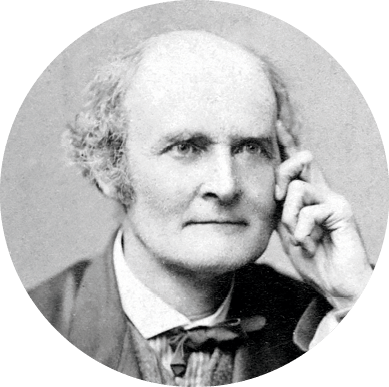
\includegraphics{images/arthur_cayley.png}
    \caption*{\centering Arthur \textsc{Cayley} (1821-1895)}
\end{marginfigure}

\begin{marginfigure}[-4cm]
    \centering
    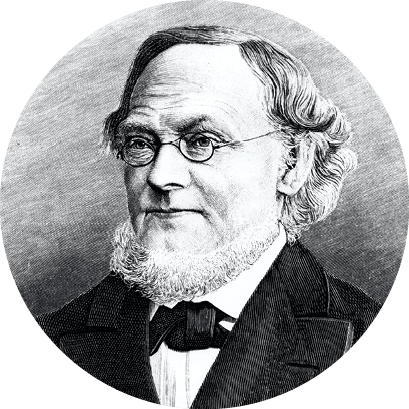
\includegraphics{images/hermann_grassmann.png}
    \caption*{\centering Hermann \textsc{Grassmann} (1809-1877)}
\end{marginfigure}